\documentclass[12pt,letterpaper]{article}
\usepackage[left=1in,right=1in, top=1in, bottom=1in]{geometry}
\usepackage[small, bf]{caption}
\usepackage[english]{babel}
\usepackage{datetime}
\usepackage{setspace}
\usepackage[pdftex]{graphicx}
\usepackage{indentfirst}
\usepackage{url}
\usepackage{minted}


\renewcommand{\theFancyVerbLine}{\sffamily
\textcolor[rgb]{0.5,0.5,1.0}{\scriptsize
\oldstylenums{\arabic{FancyVerbLine}}}}


%--------------------------------TITLE PAGE--------------------------------%

\begin{document}

\begin{titlepage}

\begin{center}

{\LARGE ASSIGNMENT 0: DSP-Experiments}
\vspace{.5 cm}

\textsc{\Large Final Project}
\vspace{1 cm}

\textsc{\Huge Avrutin, Perr-Sauer}
\vspace{.5 cm}

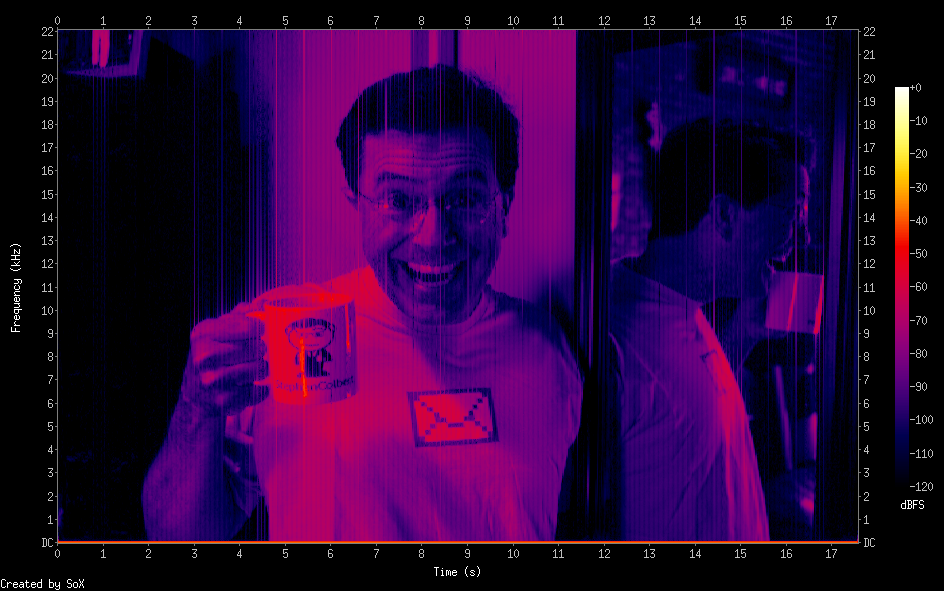
\includegraphics[scale=0.4]{../outputs/cpu_grayscale_sox.png}

\end{center}
\vfill

\begin{flushright}
\begin{large}
CS102 \\
Nicolas Avrutin, \\
2014 EE \\
\url{nicolasavru@gmail.com} \\
\vspace{.5 cm}

CS102 \\
Jordan Perr-Sauer \\
2014 EE \\
\url{jordan@jperr.com}
\vspace{.5 in}

\today

\end{large}
\end{flushright}
\end{titlepage}

\vspace{1in}
\doublespacing


%--------------------------------IDENTIFICATION-----------------------------%
\noindent
\today
\vspace{1cm}

\noindent
Jordan Perr-Sauer\\
Class of 2014\\
Electrical Engineering\\
\url{jordan@jperr.com}\\

\noindent
Nicolas Avrutin\\
Class of 2014\\
Electrical Engineering\\
\url{nicolasavru@gmail.com}\\

\noindent
Stack Overflow\\
\url{http://stackoverflow.com/questions/2063284/what-is-the-easiest-way-to-read-wav-files-using-python-summary}

\noindent
Scott Wilson, Stanford University\\
\url{https://ccrma.stanford.edu/courses/422/projects/WaveFormat/}


%--------------------------------DESCRIPTION--------------------------------%

\section{Description}

DSP-Experiments consists of python scripts that can encode images into sound files such that the image can be seen in the spectrogram of the produced sound. The code also provides a method for viewing the spectrogram of the generated audio, decoding the sound back into a (lossy) version of the original image.

In our spectrograms, the x-axis represents time (in the audio file) and the y-axis represents frequency. The brightness of a given pixel represents amplitude (loudness). To encode an image such that it can be viewed in a spectrogram, we first separate the image by it's columns of pixels. Each column of pixels will be represented by a ``tone'' in the output audio stream that lasts for a fixed amount of time. These tones consist of sin waves of varying frequencies, at varying amplitudes, depending on the intensity and position of each pixel in the column, respectively. Each column in the input image is converted into such a tone, and these tones are concatenated and output to a wave file.


%--------------------------------Compilation--------------------------------%

\section{Compilation}

You do not need to compile any part of this program. There are some dependencies, however, which you must install prior to execution.

\subsection{Dependencies}

\begin{itemize}
\item Python 2.6 or higher (NumPy and PIL are not yet compatible with Python 3)
\item NumPy (http://numpy.scipy.org/)
\item Python Imaging Library (http://www.pythonware.com/products/pil/)
\end{itemize}
%--------------------------------Execution--------------------------------%

\section{Execution}
\subsection{Manual Page}
\noindent
To produce sound (as a wav file) from an image:

\verb!python imageToWav.py g|c pathToImage pathToWav!

\noindent
The g and c options stand for ``Grayscale'' or ``Color''. Using the c option will result in a 3 channel wav file, where each channel of audio represents one channel of color (red, green, and blue). Using the g option will result in a single channel (mono) wav file and all color data will be lost.

\noindent
To generate the spectrogram of a produced (or other) wav file:

\verb!python wavToImage.py pathToWav pathToImage!

\noindent
The format of the image will be derived from the extension you give pathToImage. You can use any format supported by PIL.

\subsection{Sample Inputs}
\noindent
Sample images are provided in the test\_images dir: \\
\verb!python imageToWav.py c test_images/test.png out.wav!

\noindent
Sample wav files generate with our script are located in outputs: \\
\verb!python wavToImage.py outputs/cpu_color.wav out.png!

%--------------------------------Features--------------------------------%

\section{Features}

We support color images by using 3-channel wav files. You can specify grayscale or color using command line arguments at execution. This is discussed in ``Execution.''

%--------------------------------Notes--------------------------------%

\section{Notes}

\begin{itemize}
\item Scaling and resizing algorithms will be significantly reworked in the future.
\end{itemize}
\newpage

%--------------------------------Listings-------------------------------%

\section{Listings}
\subsection{imageToWav.py}
\inputminted[baselinestretch=1,fontsize=\footnotesize,linenos=true,fontfamily=courier]{python}{../imageToWav.py}
\newpage
\subsection{wavToImage.py}
\inputminted[baselinestretch=1,fontsize=\footnotesize,linenos=true,fontfamily=courier]{python}{../wavToImage.py}


\end{document}
